\documentclass{beamer}
% Use DS9 global theme (includes pgfplots for visualization)
\usepackage{../../../shared/templates/ds9_theme}
\usepackage{listings}
\usepackage{xcolor}

% Image path configuration
\graphicspath{{../images/}}

% C++ code listing style
\lstdefinestyle{cppstyle}{
language=C++,
backgroundcolor=\color{black!5},
commentstyle=\color{green!60!black},
keywordstyle=\color{blue},
numberstyle=\tiny\color{gray},
stringstyle=\color{purple},
basicstyle=\ttfamily\footnotesize,
breakatwhitespace=false,
breaklines=true,
captionpos=b,
keepspaces=true,
numbers=left,
numbersep=5pt,
showspaces=false,
showstringspaces=false,
showtabs=false,
tabsize=2
}
\lstset{style=cppstyle}

% Title page configuration
\title[Intro to C++]{MACS12: Introduction}
\subtitle{A Gentle Introduction to C++}
\author[Mr. Gullo]{Mr. Gullo}
\date[Aug 31, 2025]{August 31, 2025}

\begin{document}

\frame{\titlepage}

\begin{frame}
\frametitle{Learning Objectives}
\framesubtitle{Based on Today's Outline}
\begin{itemize}
\item Go over the course outline.
\item Find and install a C++ Integrated Development Environment (IDE) on your personal computers/tablets.
\item Run our first C++ program.
\item Learn about the general structure of a C++ program.
\end{itemize}
\end{frame}

\section{IDE Setup}

\begin{frame}
\frametitle{Integrated Development Environment (IDE)}
\framesubtitle{For Windows Users}
\begin{itemize}
\item \alert{Recommended:} Code::Blocks
\item We will be using Code::Blocks on the school computers and for in-class demonstrations.
\item \textbf{How to install:}
\begin{enumerate}
\item Go to \alert{codeblocks.org}.
\item Download the binary release.
\item \alert{Crucial:} Choose the file that includes mingw-setup.exe. This version includes the compiler.
\item Once installed, you may need to go to \texttt{Settings > Compiler > Toolchain executables} and click \texttt{Autodetect}.
\end{enumerate}
\end{itemize}
\end{frame}

\begin{frame}
\frametitle{IDE Setup}
\framesubtitle{For Other Platforms}
\begin{columns}[T]
\begin{column}{0.5\textwidth}
\textbf{Mac Users}
\begin{itemize}
\item The most common choice is \alert{Xcode}, available from the App Store.
\item It's a powerful, full-featured IDE from Apple.
\end{itemize}
\pause
\textbf{Android Users}
\begin{itemize}
\item \alert{C4Droid} is a solid option.
\item It may ask you to install a GCC plugin; choose "yes".
\item Other options may exist but might be paid or contain ads.
\end{itemize}
\end{column}
\begin{column}{0.5\textwidth}
\textbf{iPad Users}
\begin{itemize}
\item Options are more limited.
\item Search for "Mobile C, C/C++ Program Compiler for iOS" or similar apps.
\item A web-based IDE like \texttt{replit.com} might be a better alternative.
\end{itemize}
\end{column}
\end{columns}
\end{frame}

\section{Our First Program}

\begin{frame}[fragile]
\frametitle{Our First C++ Program: "Hello, World!"}
This is the traditional first program for any new language. It simply prints "Hello World" to the screen.

\begin{lstlisting}
#include <iostream>

using namespace std;

int main(){
cout << "Hello World" << endl;
return 0;
}
\end{lstlisting}
\end{frame}

\begin{frame}
\frametitle{Context: Creating a New Program File}
\begin{itemize}
\item Now, let's walk through the steps to create, write, and run this program in Code::Blocks.
\item The process is similar in most IDEs. You'll generally look for options like "New File" or "New Project".
\item The following slides show the specific steps for Code::Blocks.
\end{itemize}
\end{frame}

\begin{frame}
\frametitle{Visualization: New File in Code::Blocks}
\begin{figure}
\centering
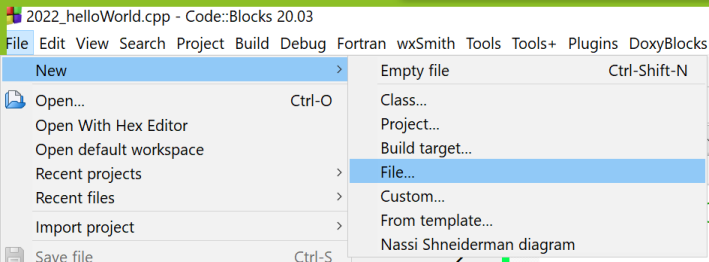
\includegraphics[width=0.8\linewidth]{cs12-codeblocks-file-new-menu.png}
\caption{Step 1: Navigate to the New File menu.}
\end{figure}
\end{frame}

\begin{frame}
\frametitle{Visualization: Choose File Type}
\begin{figure}
\centering
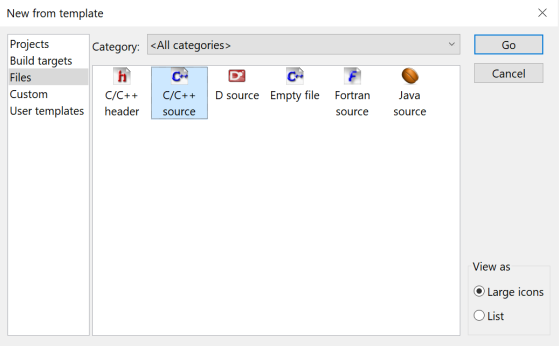
\includegraphics[width=0.8\linewidth]{cs12-codeblocks-new-from-template.png}
\caption{Step 2: Select "C/C++ source" as the file type.}
\end{figure}
\end{frame}

\begin{frame}
\frametitle{Visualization: Select Language}
\begin{figure}
\centering
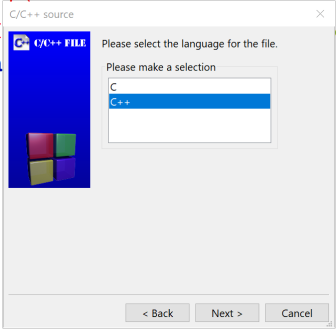
\includegraphics[width=0.8\linewidth]{cs12-codeblocks-language-selection.png}
\caption{Step 3: Make sure to select C++ as the language.}
\end{figure}
\end{frame}

\begin{frame}
\frametitle{Context: Compiling and Running}
\begin{itemize}
\item Once you've typed your code into the new file, you need to compile and run it.
\item \textbf{Compiling} turns your human-readable C++ code into machine code that the computer can execute.
\item \textbf{Running} executes that machine code.
\item Most IDEs have a single button that does both steps, often called "Build and Run".
\end{itemize}
\end{frame}

\begin{frame}
\frametitle{Visualization: Build and Run}
\begin{figure}
\centering
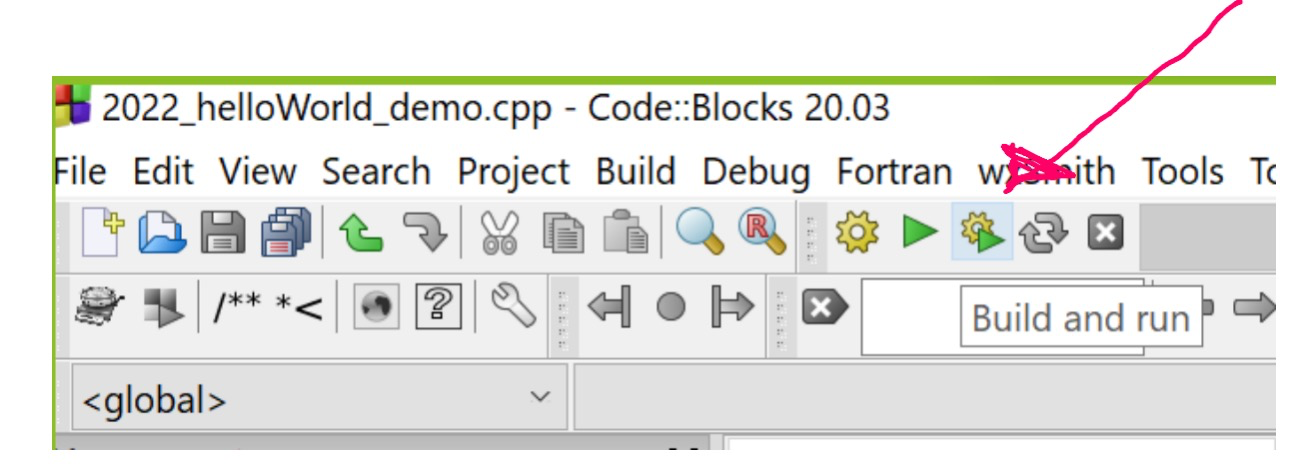
\includegraphics[width=0.9\linewidth]{cs12-codeblocks-build-and-run.png}
\caption{This button compiles your code and runs the resulting program.}
\end{figure}
\end{frame}

\begin{frame}
\frametitle{Visualization: Program Output}
\begin{figure}
\centering
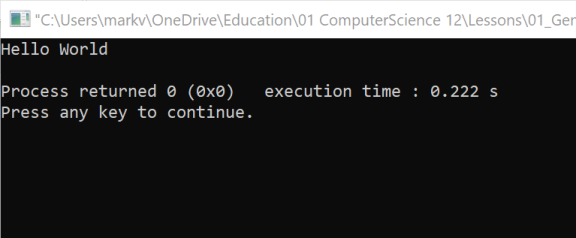
\includegraphics[width=0.8\linewidth]{cs12-console-hello-world-output.png}
\caption{The output appears in a new window called the console or terminal.}
\end{figure}
\end{frame}

\section{C++ Program Structure}

\begin{frame}
\frametitle{Why C++?}
\begin{itemize}
\item \textbf{Industry Standard:} It is still widely used by many companies for performance-critical applications like game engines, operating systems, and high-frequency trading.
\pause
\item \textbf{Power and Control:} Although it is a high-level language (like Python), it allows for low-level memory manipulation. This will be very useful for understanding some deeper computer science topics.
\end{itemize}
\end{frame}

\begin{frame}
\frametitle{The 5 Parts of a C++ Program}
\begin{itemize}
\item C++ programs generally consist of 5 different parts.
\item Understanding this structure helps in reading and writing any C++ program.
\item Let's examine them using a slightly more complex example.
\end{itemize}
\end{frame}

\begin{frame}[fragile]
\frametitle{Example Program: Area of a Circle}
\begin{lstlisting}
#include <iostream>
using namespace std;

const float pi = 3.14159;

// this function calculates the area of a circle
float circle_area(float radius)
{
return pi * radius * radius;
}

int main()
{
float diameter = 13.5;
    
cout << "The area of a circle with diameter "
     << diameter << " is " << circle_area(diameter/2)
     << endl;

return 0;
}
\end{lstlisting}
\end{frame}

\begin{frame}[fragile]
\frametitle{Part 1: Pre-processor Directives}
These lines give the compiler information it needs to read your program.
\begin{lstlisting}
#include <iostream>
using namespace std;
\end{lstlisting}
\begin{itemize}
\item \texttt{#include <iostream>}: Includes the input-output stream library, which lets us use \texttt{cout}.
\item \texttt{using namespace std;}: Tells the compiler we are using elements from the standard library (like \texttt{cout} and \texttt{endl}).
\end{itemize}
\end{frame}

\begin{frame}[fragile]
\frametitle{Part 2: Constant Definitions}
This section contains name-value pairs that will not change during the program's execution.
\begin{lstlisting}
const float pi = 3.14159;
\end{lstlisting}
\begin{itemize}
\item The \texttt{const} keyword ensures that the value of \texttt{pi} cannot be accidentally changed later in the program.
\item This is useful for values like mathematical constants or configuration settings.
\end{itemize}
\end{frame}

\begin{frame}[fragile]
\frametitle{Bonus: Comments}
Comments are notes for human readers that the compiler ignores.
\begin{lstlisting}
// This is a single-line comment.

/*
This is a
multi-line comment. Everything
between the symbols is ignored.
*/

int main(){
/*
cout << "Hello World" << endl;
cout << "Testing Comments" << endl;
*/
return 0; // This code will not run
}
\end{lstlisting}
\end{frame}

\begin{frame}[fragile]
\frametitle{Part 3: Main Body Heading}
This is the special function where your program's execution begins.
\begin{lstlisting}
int main()
{
\end{lstlisting}
\begin{itemize}
\item Every C++ program must have a \texttt{main} function.
\item The operating system calls this function when you run your program.
\item The code to be executed is placed between the curly braces \texttt{{}}.
\end{itemize}
\end{frame}

\begin{frame}[fragile]
\frametitle{Part 4: Main Body Variable Declarations}
Here, we declare variables that will be used within the main function.
\begin{lstlisting}
float diameter = 13.5;
\end{lstlisting}
\begin{itemize}
\item The syntax is \texttt{<datatype> <variablename> = <value>;}
\item This line creates a variable named \texttt{diameter} of type \texttt{float} (a number with decimals) and gives it an initial value of 13.5.
\item We'll look at data types in more detail next class.
\end{itemize}
\end{frame}

\begin{frame}[fragile]
\frametitle{Part 5: Main Body Statements}
These are the actions and instructions that make up the body of your program.
\begin{lstlisting}
cout << "The area of a circle with diameter "
<< diameter << " is " << circle_area(diameter/2)
<< endl;
return 0;

  

\end{lstlisting}
\begin{itemize}
\item \texttt{cout << ... ;}: A statement that prints text and variable values to the console.
\item \texttt{return 0;}: This is the last statement. It tells the operating system that the program finished successfully.
\end{itemize}
\end{frame}

\section{Practice}

\begin{frame}[fragile]
\frametitle{I Do: Displaying Text}
\textbf{Goal:} Write a C++ program that prints the phrase "Hello World" to the screen.

\pause

\textbf{Code Structure:}
\begin{lstlisting}
// 1. Pre-processor directives
#include <iostream>
using namespace std;
\end{lstlisting}
\pause
\begin{lstlisting}
// 2. Main function heading
int main() {
\end{lstlisting}
\pause
\begin{lstlisting}     
// 3. Main body statement
cout << "Hello World" << endl;
\end{lstlisting}
\pause
\begin{lstlisting}    
// 4. Return statement
return 0;
}
\end{lstlisting}
\textbf{Output:} The program will print \texttt{Hello World} to the console.
\end{frame}

\begin{frame}[fragile]
\frametitle{We Do: Modifying Output}
\textbf{Goal:} How would we modify our "Hello World" program to greet you by name? For example, "Hello, Mr. Gullo!"

\pause

\textbf{Code:}
\begin{lstlisting}
#include <iostream>
using namespace std;

int main() {
// What goes inside the quotes?
cout << "..." << endl;
return 0;
}
\end{lstlisting}
\pause
\vspace{1cm}
\begin{center}
\huge
\alert{\texttt{cout << "Hello, Mr. Gullo!" << endl;}}
\end{center}

\end{frame}

\begin{frame}[fragile]
\frametitle{You Do: Your First Program}
\textbf{Task:} Write a complete C++ program from scratch that does the following:
\begin{enumerate}
\item Prints your first name to the console.
\item On a \alert{new, separate line}, prints your favorite hobby.
\end{enumerate}

\pause

\textbf{Hint:} Remember what \texttt{endl} does. You can use \texttt{cout} multiple times.

\vfill
\textbf{Example Output:}
\begin{verbatim}
Mark
Confiscating Devices
\end{verbatim}
\end{frame}

\section{Summary}

\begin{frame}
\frametitle{Summary and Next Steps}
\begin{itemize}
\item \textbf{Today's Goal:} The main objective was to get a working C++ IDE installed and to run your first simple program.
\item \textbf{Program Structure:} We learned that C++ programs have a consistent structure:
\begin{enumerate}
\item Pre-processor Directives (\texttt{#include})
\item Constant Definitions (\texttt{const})
\item Main Body Heading (\texttt{int main()})
\item Variable Declarations (\texttt{float diameter;})
\item Main Body Statements (\texttt{cout}, \texttt{return})
\end{enumerate}
\item \textbf{For Extra Practice:}
\begin{itemize}
\item Project Euler (\texttt{projecteuler.net}) - Mathematical problems.
\item Waterloo Computing Challenge Questions - Logic and algorithm problems.
\end{itemize}
\end{itemize}
\end{frame}

\end{document}